\chapter{GoogLeNet}
{
\label{chap:googlenet}
本研究でマルチFPGA上に実装するアプリケーションであるGoogLeNet\cite{googlenet}について説明する.
GoogleNetは畳込みニューラルネットワーク(CNN: Convolutional Neural Network)のモデルの1つである.

\section{Convolutional Neural Network}
\label{sec:cnn}
2012年に行われた国際的な画像認識のコンペティション,ImageNet Large Scale Visual Recognition Challenge(ILSVRC)
で登場したAlexNet\cite{alexnet}が高い認識精度を出して優勝したことからCNNは特に画像認識の分野で優れた識別精度をマークすることがわかり世界で注目されるようになった.
ILSVRCでは与えられた画像に何が映っているのか,画像のどこに映っているのかなどをいかに高精度に認識させるかを競う大会である。
AlexNetのILSVRC優勝を皮切りに様々なCNNのモデルの検討,実装が行われ最新のモデルは人間の認識精度を超える精度を出すようにまでなった。
%Neural Networkの説明

\subsection{Neural Network}
\label{sec:nn}
ニューラルネットワークは動物の神経ニューロンが接続され,神経物質が伝搬されるように演算モジュールを層として複数,結合していく.
演算ネットワークでは神経物質の代わりに例えば画像における画素値のような入力ベクトルの演算結果が伝搬していく.
ニューラルネットワークでは2つの演算フェーズ,学習と推論がある.
学習では教師データ(識別された画像)をもとに各演算層のパラメータを決定する.
推論では学習で得たパラメータを用いて,入力値(未識別の画像)から演算(入力画像の識別)を行う.
本研究ではCNNの推論アクセラレータを実装するので推論演算で用いられるアルゴリズムについて説明する.

\subsection{Convolution}
\label{sec:conv}
CNNはその名前にも含まれているように式で表される畳み込み演算と呼ばれる行列の積和演算がその主なアルゴリズムである.
CNNでは各層の演算結果を次の層の入力値として受け渡す.これを特徴マップと呼ぶ.
特徴マップは学習フェーズで得られた重みフィルタと呼ばれる行列と積和演算が行われ,同じく学習フェーズで得られたバイアスと呼ばれるパラメータを加算することで
出力値を求める.
% conv
\begin{equation}
	output(f_o, x, y) = \sum_{f_i = 0}^{N_if}\sum_{k_x = 0}^{K}\sum_{k_y = 0}^{K}weight(f_o, f_i,k_x,k_y) * input(f_i,x + k_x, y + k_y) + bias(f_o, x, y)
\end{equation}
% 図\ref{fig:conv}に畳み込み演算の様子を図示する。

\subsection{Other layer calculation}
\label{sec:other_calc}
CNNには畳み込み演算の他にもいくつかの演算を必要とする。その代表的なものとして,全結合とプーリング処理がある。
これらはそれぞれ式\ref{eq:fc},式\ref{eq:pool}で表される。

% full connect
\begin{equation}
  \label{eq:fc}
  output(i) = bias(i) + \sum_{j=0}^{N} weight(i, j) * input(j)
\end{equation}

% max pool
\begin{equation}
  \label{eq:pool}
	output(x, y)^{i} = max / average(input(f_i,x + k_x, y + k_y)) (0<= (k_x, k_y) < K)
\end{equation}

全結合層では畳み込み演算同様,入力値と重みフィルタの値を乗算するところは同じである。しかし,それぞれの出力値に入力値を全てが必要という点で異なる。
また各出力層に対して入力値全てについて計算しなければいけないので畳み込み演算に比べて演算量,パラメータ数ともに大きくなってしまうという特徴もある。
プーリング層では入力特徴マップの圧縮を行う。特徴マップのそれぞれのフィルタサイズの領域内の平均値もしくは最大値を取ることで入力特徴マップの特徴はそのままに
データサイズを圧縮することができる.
これらの演算を各層で処理し伝搬していき出力されるという構造をとっている.

\section{GoogLeNet}
\label{sec:googlenet}
GoogLeNetは2014年のILSVRCで最高精度をマークし優勝したCNNモデルである.
構成要素は上述の畳み込み演算,プーリング処理などが主であるという点においてはAlexNetなどと
違いはないがそれぞれの層の接続の仕方,層の深さが異なりAlexNetに見られる全結合層がないという点で異なる.
AlexNet, GoogLeNetそれぞれについて図にその全体像を示す.


\begin{figure}[h]
  \centering
  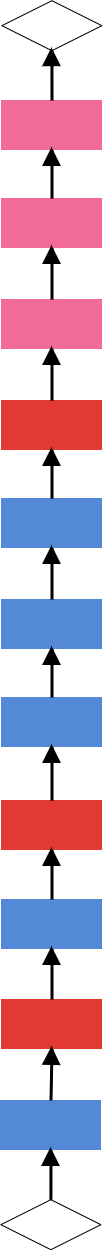
\includegraphics[scale=0.5]{./chap2/fig/alexnet.png}
  \caption{AlexNetのアーキテクチャ}
  \label{fig:alexnet}
\end{figure}

\begin{figure}[h]
  \centering
  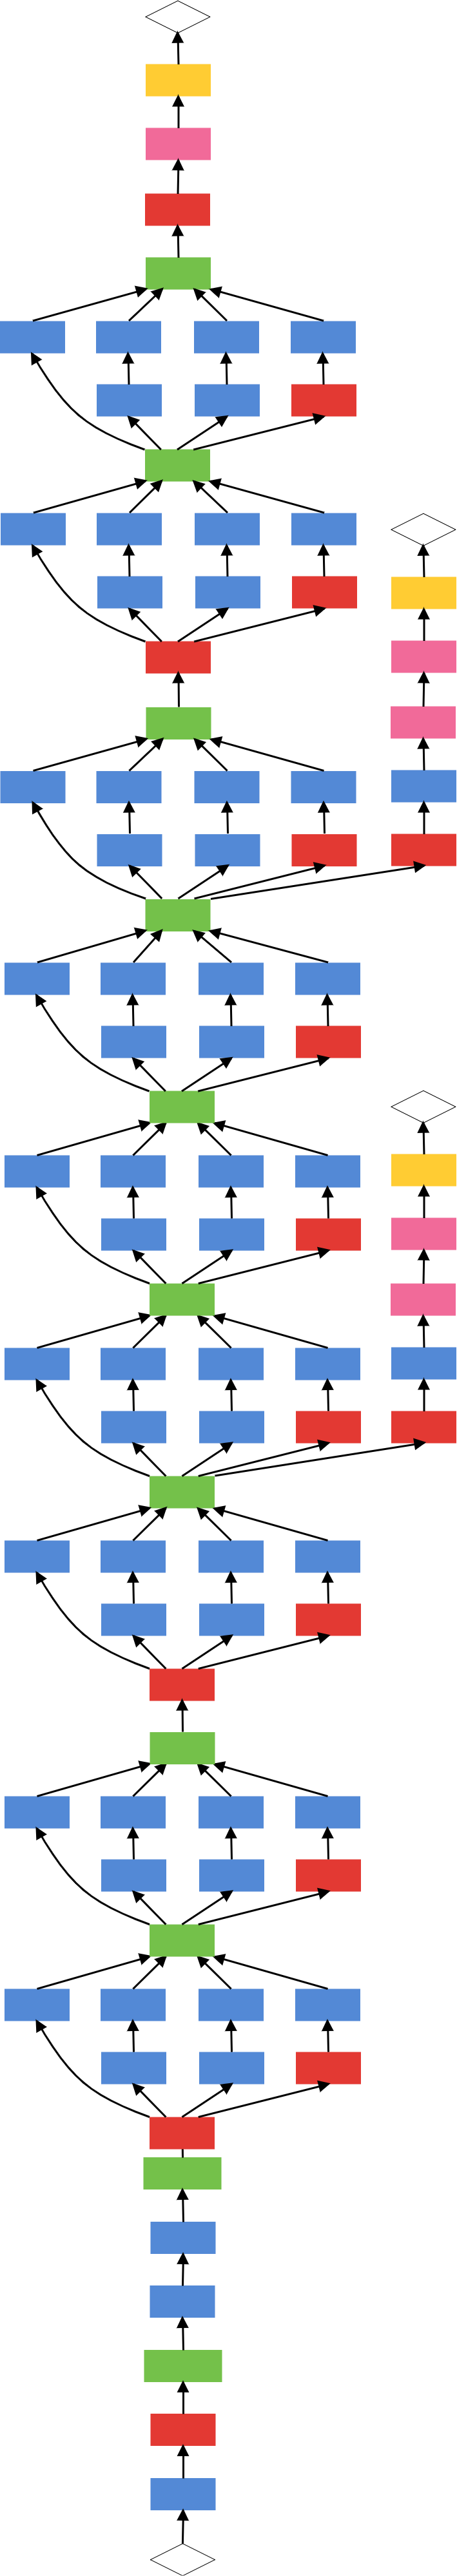
\includegraphics[scale=0.2]{./chap2/fig/googlenet.png}
  \caption{GoogLeNetのアーキテクチャ}
  \label{fig:googlenet}
\end{figure}

図\ref{fig:alexnet},\ref{fig:googlenet}のブロックはそれぞれの演算層を示している。
青のブロックは畳込み層,赤はpooling層,ピンクは全結合層,黄色はsoftmax層と呼ばれる画像分類のために用いられる。
緑のブロックはDepthConcat層で並列に処理した出力特徴マップを結合する.
両者を比較すると,GoogLeNetのほうが,層がより深くなっていること,さらに横に広がっていることがわかる.
GoogLeNetは層を深くする代わりにそのフィルタサイズを小さくすることで,計算量,メモリアクセスを減らすように設計されている.
% 〇〇の研究によると一つの大きなフィルタによる畳込みよりも複数の小さなフィルタによる畳込みのほうがより高い精度を出すことができるとされている.
さらにGoogLeNetではモデル内の横に広がった複数の層をInception層と名付け,これを複数層重ねる設計をしている.

\section{Inception}
\label{sec:inception}
Inception層は次の図で示される(これは図\ref{fig:googlenet}の一部を拡大したものと同じである)

\begin{figure}[h]
  \centering
  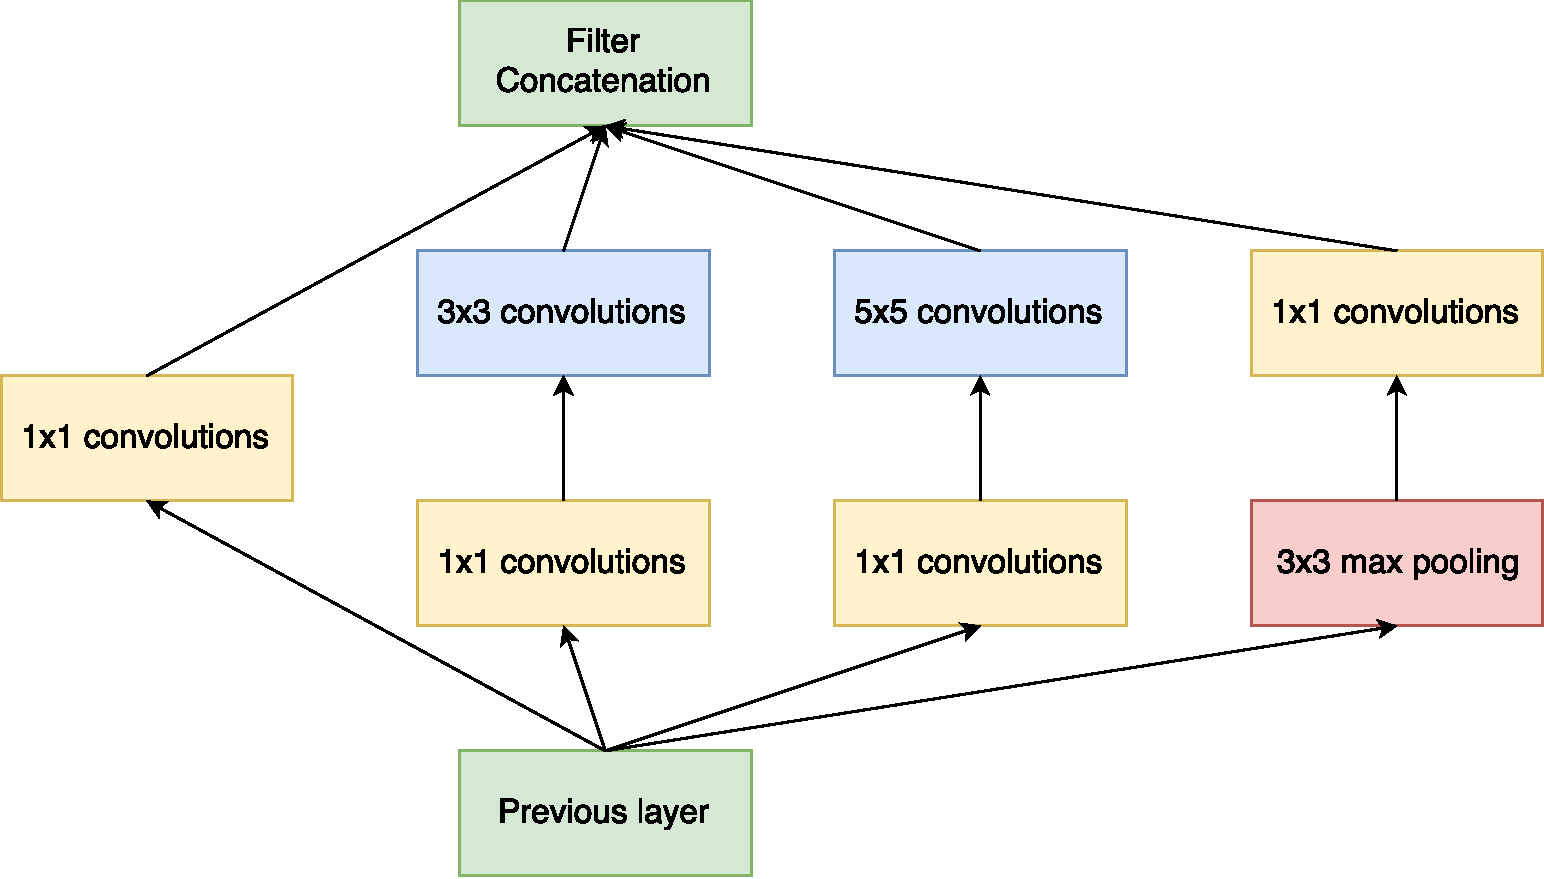
\includegraphics[scale=0.5]{./chap2/fig/inception.pdf}
  \caption{Inception層}
  \label{fig:inception}
\end{figure}

これを見ると横に広がった層の中で1$\times$1convと記されている層がある.この層ではサイズ1のフィルターを用いて,畳込み演算を行っている.
この層は,次元削減を行っている.これは入力チャネル(入力行列の深さ)に対して少ない層のフィルタを畳み込み演算することでその深さを
削減する,これによって計算量が減るだけでなく,精度向上が実現できる.
Inception層の出力の手前のDepthConcat層は図\ref{fig:googlenet}の緑のブロックで示され,
横に広がった層のそれぞれの出力結果を図\ref{fig:depthconcat}のように深さ方向に結合することで
一つの行列として出力値にまとめる処理を行っている.

\begin{figure}[h]
  \centering
  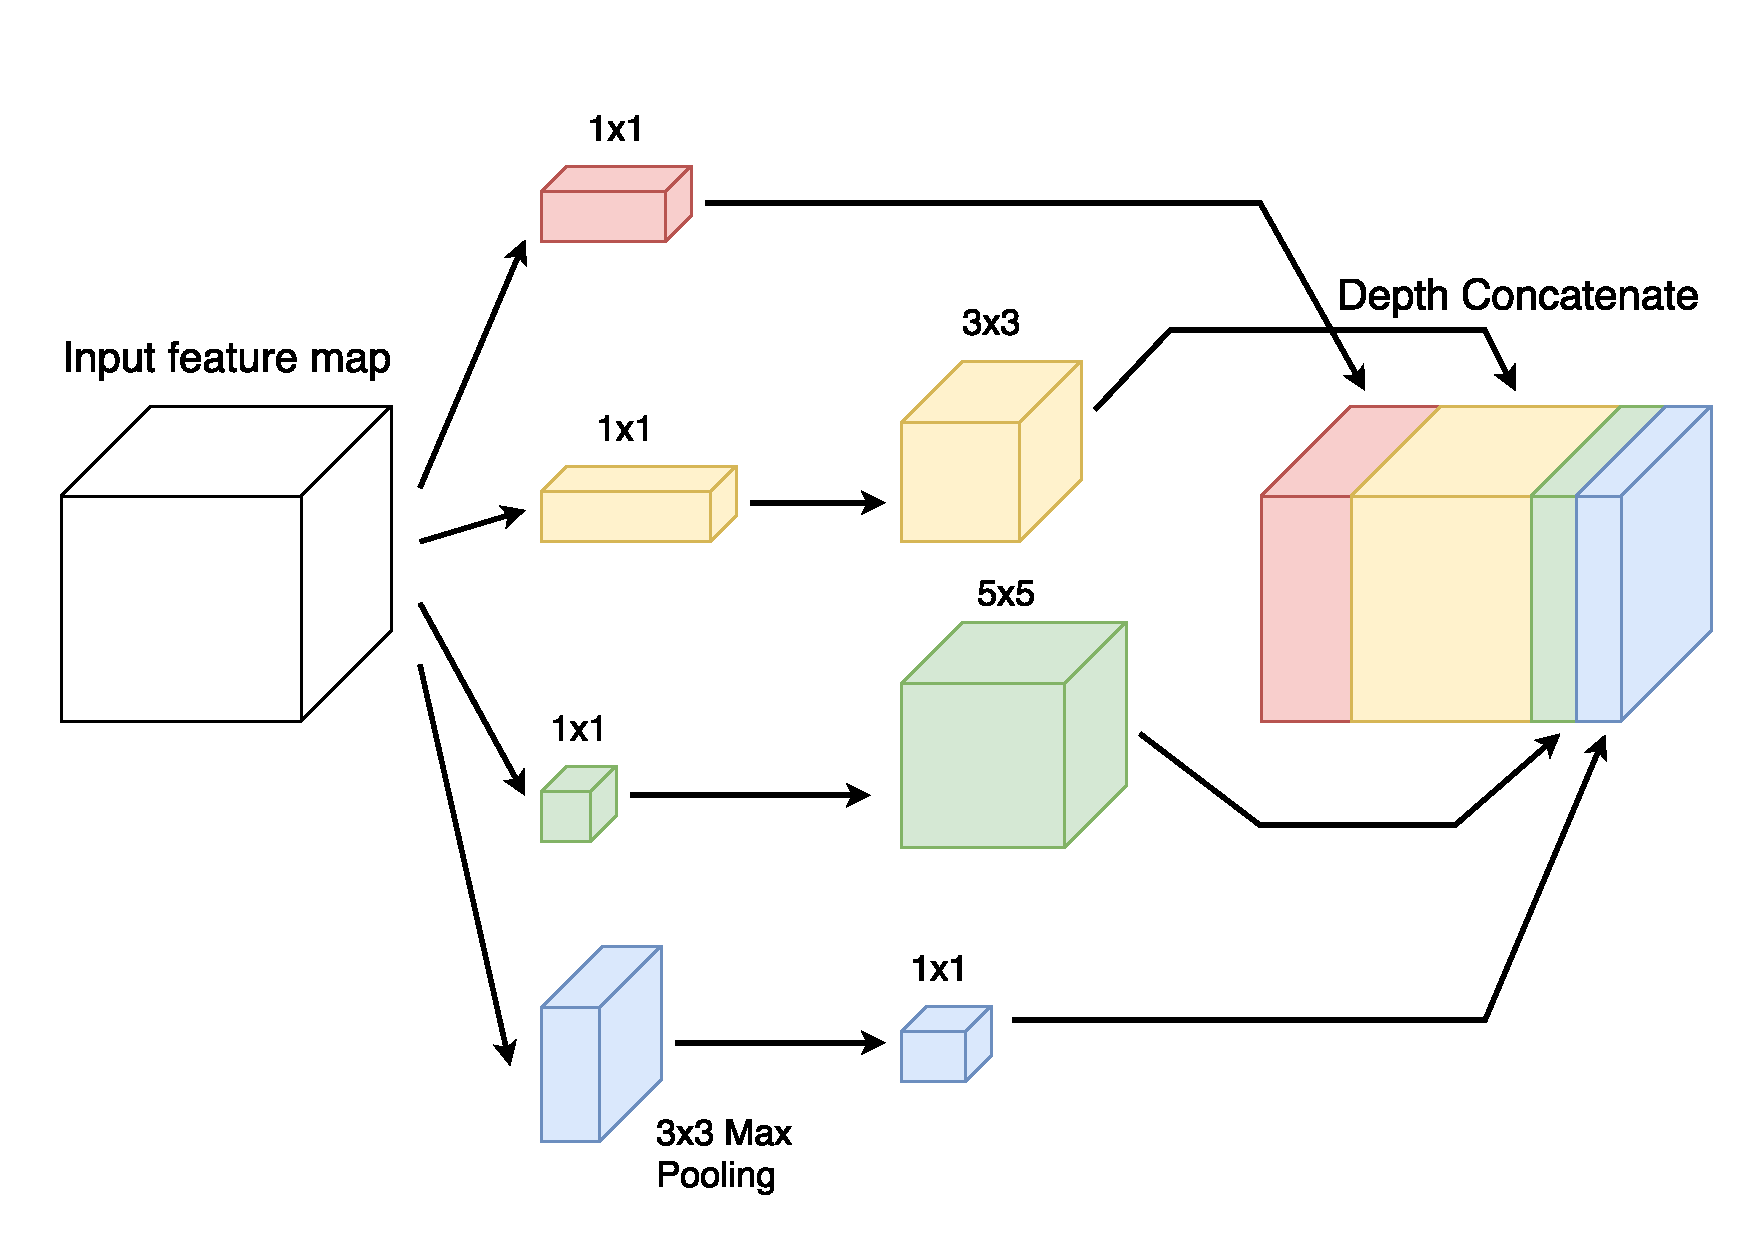
\includegraphics[scale=0.5]{./chap2/fig/depthconcat.pdf}
  \caption{DepthConcat層}
  \label{fig:depthconcat}
\end{figure}

この特徴的なInception層を積層していくことで,GoogLeNetは構成される.表\ref{table:googlenet}にGoogLeNetでの各層の入出力サイズと必要なパラメータ数をまとめる.

\begin{table}[p]
  \begin{center}
  \caption{GoogLeNetにおける各層の構成}
  \label{table:googlenet}
  \begin{tabular}{|c|c|c|c|c|c|c|c|c|c|c|} \hline
  \multicolumn{1}{|c|}{type} & \multicolumn{1}{|c|}{\shortstack{patch size/\\ stride}} & \multicolumn{1}{|c|}{\shortstack{output\\ size}} & \multicolumn{1}{|c|}{\#1$\times$1} & \multicolumn{1}{|c|}{\shortstack{\#3$\times$3\\ reduce}} & \multicolumn{1}{|c|}{\#3$\times$3} & \multicolumn{1}{|c|}{\shortstack{\#5$\times$5\\ reduce}} & \multicolumn{1}{|c|}{\#5$\times$5} & \multicolumn{1}{|c|}{\shortstack{pool\\ proj}} & \multicolumn{1}{|c|}{params} & \multicolumn{1}{|c|}{ops} \\ \hline \hline
  convolution    & 7$\times$7/2 & 112$\times$112$\times$64  &  &  &  &  &  &  & 2.7K & 34M \\ \hline
  max pool       & 3$\times$3/2 & 56$\times$56$\times$64  &  &  &  &  &  &  &  &  \\ \hline
  convolution    & 3$\times$3/1 & 56$\times$56$\times$192  &  & 64 & 192 &  &  &  & 112K & 360M  \\ \hline
  max pool       & 3$\times$3/2 & 28$\times$28$\times$192  &  &  &  &  &  &  &  & \\ \hline
  inception (3a) &  & 28$\times$28$\times$256  & 64 & 96 & 128 & 16 & 32 & 32 & 159K & 128M \\ \hline
  inception (3b) &  & 28$\times$28$\times$480  & 128 & 128 & 192 & 32 & 96 & 64 & 380K & 304M \\ \hline
  max pool       & 3$\times$3/2 & 14$\times$14$\times$480  &  &  &  &  &  &  &  &  \\ \hline
  inception (4a) &  & 14$\times$14$\times$512 & 192 & 96 & 208 & 16 & 48 & 64 & 364K & 73M \\ \hline
  inception (4b) &  & 14$\times$14$\times$512 & 160 & 112 & 224 & 24 & 64 & 64 & 437K & 88M \\ \hline
  inception (4c) &  & 14$\times$14$\times$512 & 128 & 128 & 256 & 24 & 64 & 64 & 463K & 100M \\ \hline
  inception (4d) &  & 14$\times$14$\times$528 & 112 & 144 & 288 & 32 & 64 & 64 & 580K & 119M \\ \hline
  inception (4e) &  & 14$\times$14$\times$832 & 256 & 160 & 320 & 32 & 128 & 128 & 840K & 170M \\ \hline
  max pool       & 3$\times$3/2 & 7$\times$7$\times$832 &  &  &  &  &  &  &  &  \\ \hline
  inception (5a) &  & 7$\times$7$\times$832 & 256 & 160 & 320 & 32 & 128 & 128 & 1072K & 54M \\ \hline
  inception (5b) &  & 7$\times$7$\times$1024 & 384 & 192 & 384 & 48 & 128 & 128 & 1388K & 71M \\ \hline
  avg pool       & 7$\times$7/1 & 1$\times$1$\times$1024 &  &  &  &  &  &  &  &  \\ \hline
  dropout (40\%) &  & 1$\times$1$\times$1024 &  &  &  &  &  &  &  &  \\ \hline
  linear         &  & 1$\times$1$\times$1000 &  &  &  &  &  &  & 1000K & 1M \\ \hline
  softmax        &  & 1$\times$1$\times$1000 &  &  &  &  &  &  &  &  \\ \hline
  \end{tabular}
  \end{center}
\end{table}
  
それぞれのInception層はサイズは異なるが,図\ref{fig:inception}に示す構造を取っている.
表\ref{table:googlenet}中の\#3$\times$3reduceや\#5$\times$5reduceは3$\times$3や5$\times$5の畳み込み演算の前に行われる1$\times$1の畳み込み演算の重みの深さを示している。
またpool projも同じようにmax poolの後に行われる,1$\times$1の畳み込み演算層の重みフィルタの深さを示している.
この表を見るとAlexNetに見られるような全結合層がないことがわかる.GoogLeNetでは計算量の多い全結合層を
削除することで全体の計算量を減らしながら高い精度を保っている.
}